\section{Sampling Error and Overfitting}
\label{sec:overfitting}

%A second source of error in minimizing the Bellman error, orthogonal to function approximation, is that of sampling or generalization error. The next issue we investigate is the effect of sampling error on Q-learning methods.

%\subsection{Technical Background}
\begin{wrapfigure}{r}{0.6\columnwidth}
\centering
\vspace{-10pt}
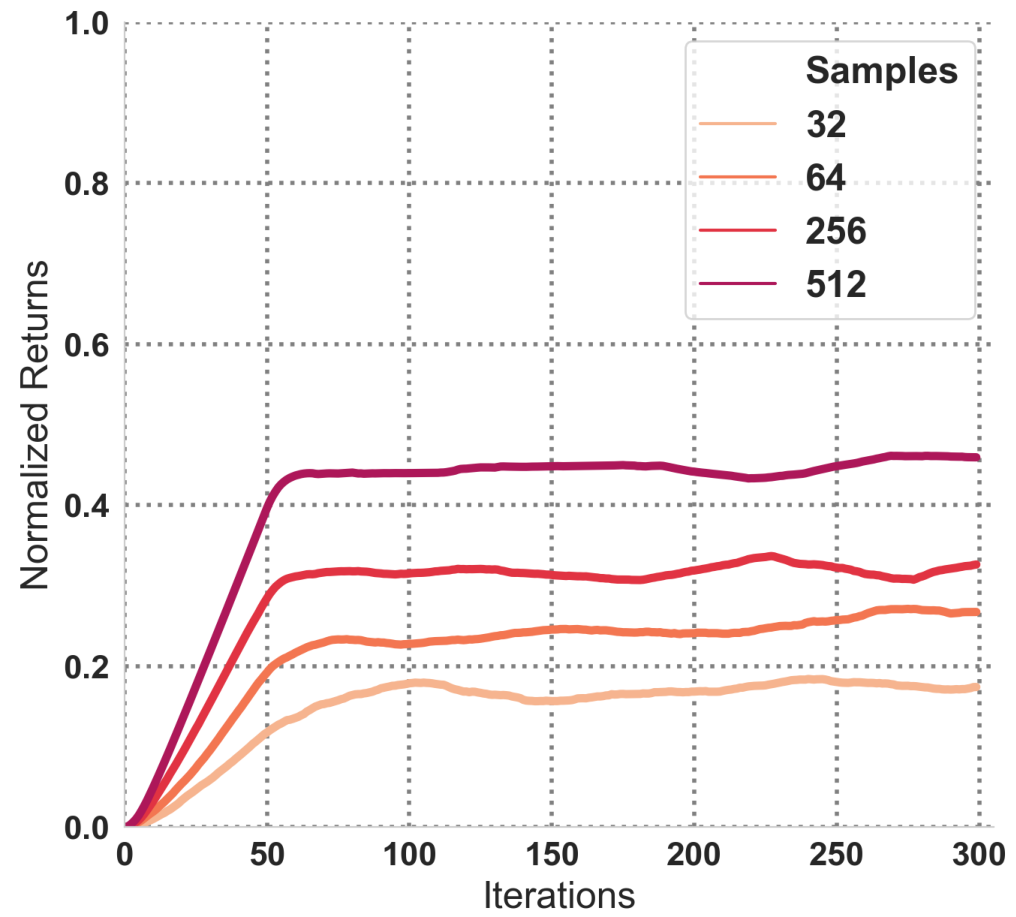
\includegraphics[scale=0.27]{chapters/diagnosing_q/images/samples_arch.pdf}
\vspace{-0.2cm}
\caption{\label{fig:sampling_256} Samples plotted with returns for a 256x256 network. More samples yields better performance.}
\vspace{-0.6cm}
%plot_sampling
%east1//2019-01-20-newenv-sample-weighting
\end{wrapfigure}

Approximate dynamic programming assumes that the projection of the Bellman backup (Eqn.~\ref{eqn:bellman_projection}) is computed exactly, but in reinforcement learning we can normally only compute the \textit{empirical Bellman error} over a finite set of samples. In the PAC framework, overfitting can be quantified by a bounded error in between the empirical and expected loss with high probability, which decays with sample size~\citep{Shalev2014}. \citet{munos2008finite, maillard2010finite, tosatto2017boosted} provide such PAC-bounds which account for sampling error in the context of Q-learning and value-based methods, and quantify the quality of the final solution in terms of sample complexity.

We analyze several key points that relate to sampling error. First, we show that Q-learning is prone to overfitting, and that this overfitting has a real impact on performance. We also show that the replay buffer is in fact an effective technique in addressing this issue, and discuss several methods to migitate the effects of overfitting in practice.

\subsection{Quantifying Overfitting}
We first quantify the amount of overfitting that happens during training, by varying the number of samples. In order provide comparable validation errors across different experiments, we fix a reference sequence of Q-functions, $Q^1, ... , Q^N$, obtained during an arbitrary run of FQI. We then retrace the training sequence, and minimize the projection error $\Projmu(Q^t)$ at each training iteration, using varying amounts of on-policy data or sampling from a replay buffer. We measure the validation error (the expected Bellman error) at each iteration under the on-policy distribution, plotted in Fig.~\ref{fig:sampling_validation_loss}. We note the obvious trend that more samples leads to significantly lower validation loss. A more interesting observation is that sampling from the replay buffer results in the lowest on-policy validation loss, despite bias due to distribution mismatch from sampling off-policy data. As we elaborate in Section~\ref{sec:analysis_nonstationarity}, we believe that replay buffers are effective because they reduce overfitting and have good sample coverage over the state space, not necessarily due to reducing the effects of nonstationarity.

Next, Fig.~\ref{fig:sampling_256} shows the relationship between number of samples and returns. We see that more samples leads to improved learning speed and a better final solution. A full sweep including architectures is presented in Appendix Fig.~\ref{fig:sampling_arch_sweep}. Despite overfitting being an issue, larger architectures still perform better because the bias introduced by smaller architectures dominates.

\begin{figure*}[ttt!]
\begin{minipage}[t]{0.32\linewidth}

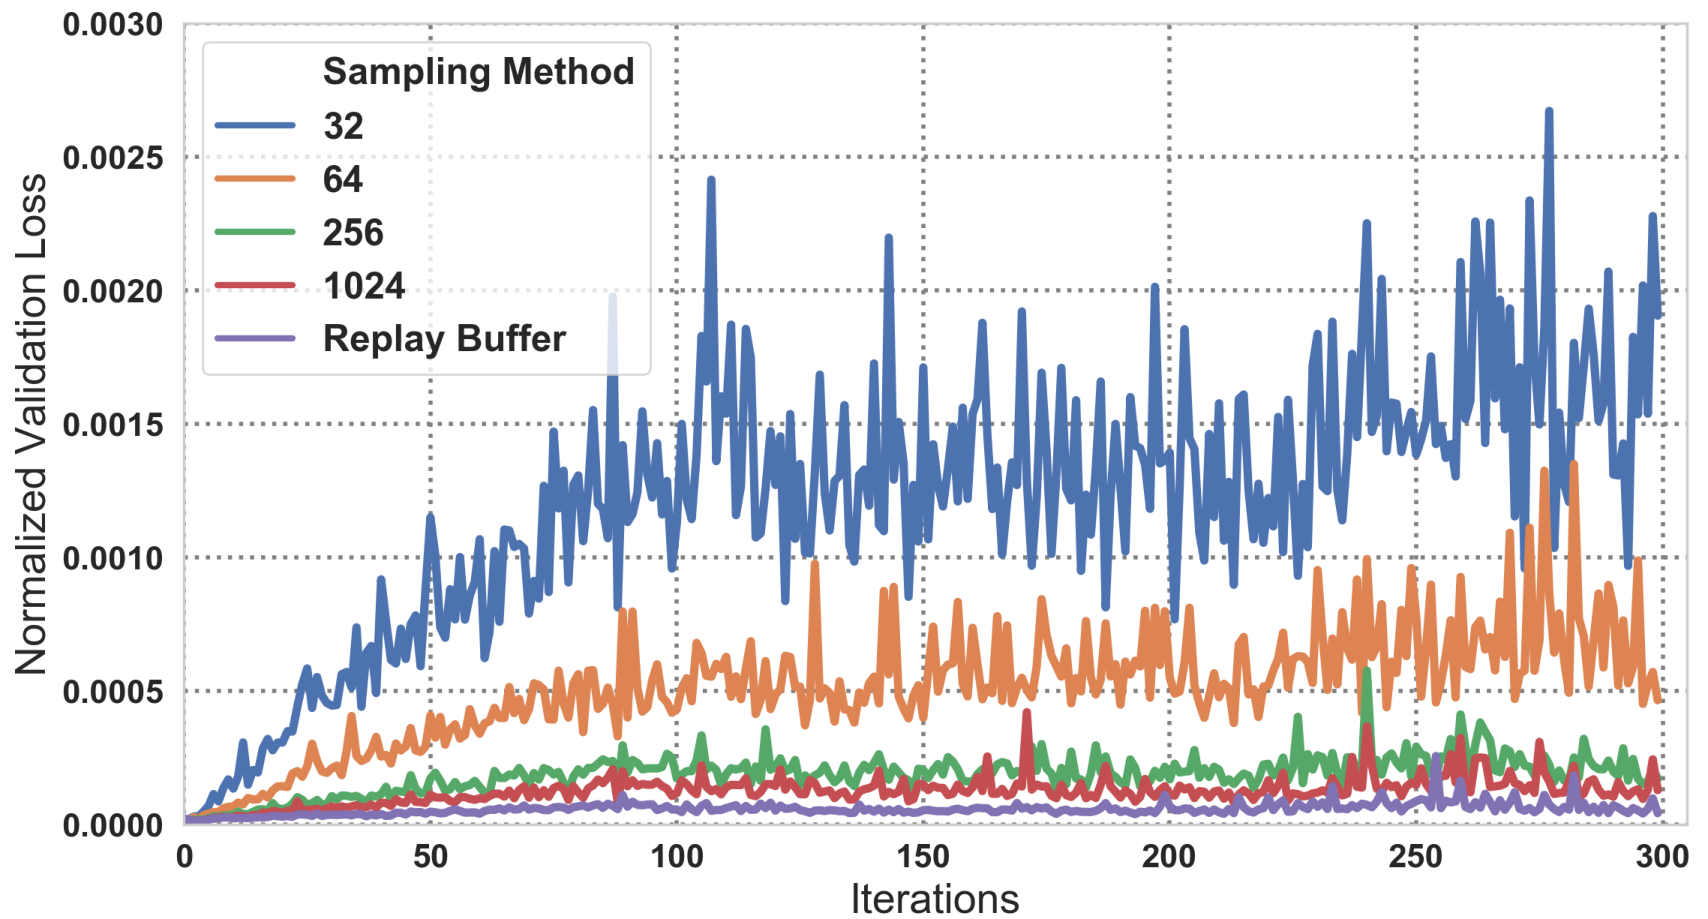
\includegraphics[width=0.95\columnwidth]{chapters/diagnosing_q/images/overfitting.pdf}
%plot_overfitting
%central1//2019-01-21-overfitting-coupled
\caption{\label{fig:sampling_validation_loss} On-policy validation losses for varying amounts of on-policy data (or replay buffer), averaged across environments and seeds. Note that sampling from the replay buffer has lower on-policy validation loss, despite bias from distribution shift.}
\end{minipage}
~\vline~
\begin{minipage}[t]{0.32\linewidth}
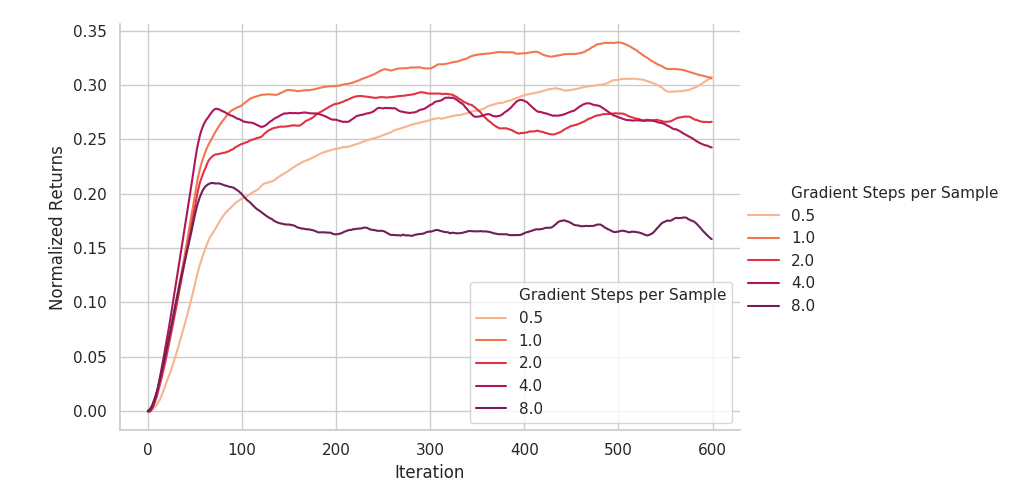
\includegraphics[trim={0 0 7.0cm 0},clip,width=0.95\columnwidth]{chapters/diagnosing_q/images/grad_steps_fqi}
%plot_overfitting
%central1//2019-01-21-overfitting-coupled
\caption{\label{fig:fqi_grad_sweep}Normalized returns plotted over training iterations (32 samples are taken per iteration), for different ratios of gradient steps per sample using Replay-FQI. We observe that intermediate values of gradient steps work best, and too many gradient steps hinders performance.}
\end{minipage}
~\vline~
\begin{minipage}[t]{0.32\linewidth}
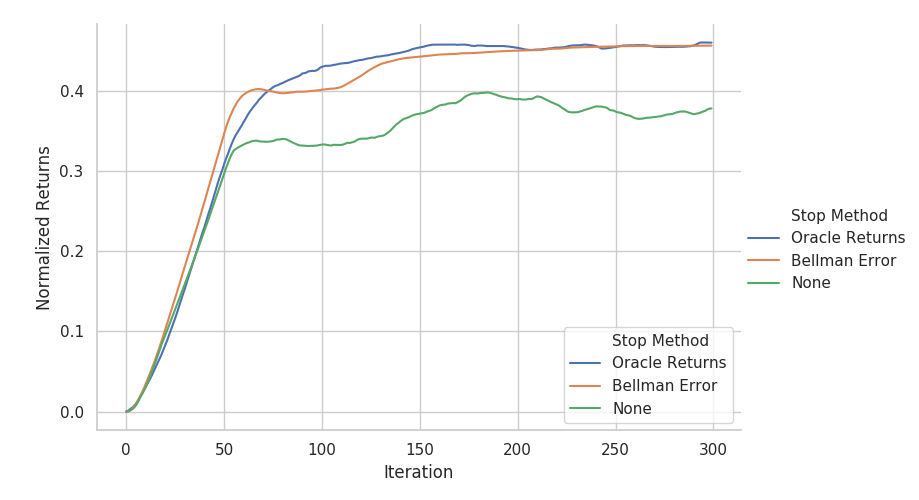
\includegraphics[trim={0 0 4.4cm 0},clip,width=0.95\columnwidth]{chapters/diagnosing_q/images/validation_stop}
%plot_validation_stop
%west1//2019-02-20-replay-validation-stop
\caption{\label{fig:validation_stop}Normalized returns plotted over training iterations (32 samples are taken per iteration), for different early stopping methods using Replay-FQI. We observe that using proper early stopping can result in a modest performance increase.}
\end{minipage}
\end{figure*}

\subsection{How can we compensate for overfitting?}

Finally, we discuss methods to compensate for overfitting. One common method for reducing overfitting is to regularize the function approximator to reduce its capacity. However, we have seen that weaker architectures can give rise to suboptimal convergence. Instead, we study \textit{early stopping} methods to mitigate overfitting without reducing model size.
We first note that the number of gradient steps taken per sample in the projection step has an important effect on performance -- too few steps and the algorithm learns slowly, but too many steps and the algorithm may initially learn quickly but overfit. To show this, we run an ablation over the number of gradient steps taken per sample in Replay-FQI and TD3 (TD3 uses 1 by default). Results for FQI are shown in Fig.~\ref{fig:fqi_grad_sweep}, and for TD3 in Appendix Fig.~\ref{fig:td3_grad_sweep}.

In order to understand whether early stopping criteria can reduce overfitting, we employ \emph{oracle} stopping rules to provide an ``upper bound'' on the best potential improvement. We try two criteria for setting the number of gradient steps: the expected Bellman error and the expected returns of the greedy policy (oracle returns). We implement both methods by running the projection step of FQI to convergence, and retroactively selecting the intermediate Q-function which is judged best by the evaluation metric. Using oracle stopping metrics results in a modest boost in performance in tabular domains (Fig.~\ref{fig:validation_stop}). Thus, we believe that there is promise in further improving such early-stopping methods for reducing overfitting in deep RL algorithms.

We can draw a few conclusions from these experiments. First, overfitting is indeed an issue with Q-learning, and too many gradient steps or too few samples can lead to poor performance. Second, replay buffers and early stopping can mitigate the effects of overfitting. Third, although overfitting is a problem, large architectures are still preferred, because the bias from function approximation outweighs the increased overfitting from using large models.